\documentclass[cs4size,a4paper]{ctexart}   
\newcommand{\subsubsubsection}[1]{\paragraph{#1}\mbox{}\\}
\setcounter{secnumdepth}{4} % how many sectioning levels to assign numbers to
\setcounter{tocdepth}{4} % how many sectioning levels to show in ToC

%===数学符号公式===
\usepackage{amsmath}    					% AMS LaTeX宏包
\usepackage[style=1]{mdframed}
\usepackage{amsthm}
\usepackage{amssymb}
\usepackage{bm}                      	% 数学公式中的黑斜体
\usepackage{bbm}
\usepackage{amsfonts}
\usepackage{mathrsfs}                	% 英文花体字 体
\usepackage{bbding,manfnt}    			% 一些图标,如 \dbend
\usepackage{lettrine}                	% 首字下沉,命令\lettrine
\def\attention{\lettrine[lines=2,lraise=0,nindent=0em]{\large\textdbend\hspace{1mm}}{}}
\usepackage{longtable}
\usepackage{enumerate}
\usepackage[toc,page]{appendix}
\usepackage{geometry}         			% 页边距调整
\geometry{top=3.0cm,bottom=2.7cm,left=2.5cm,right=2.5cm}
\usepackage[colorinlistoftodos,prependcaption,textsize=small]{todonotes}
%===公式按章编号===
\numberwithin{equation}{section}
\numberwithin{table}{section}
\numberwithin{figure}{section}
%===基本格式预置===
\usepackage{fancyhdr}
\pagestyle{fancy}
\fancyhf{}  
\fancyhead[C]{\zihao{5}  \kaishu LaTeX软件使用指导}
\fancyfoot[C]{~\zihao{5} \thepage~}
\renewcommand{\headrulewidth}{0.75pt} 
\CTEXsetup[format={\centering\bfseries\zihao{-2}},name={第, 章}]{section}
\CTEXsetup[nameformat={\bfseries\zihao{3}}]{subsection}
\CTEXsetup[nameformat={\bfseries\zihao{4}}]{subsubsection}
%===图形支持宏包===
\usepackage{graphicx}        			% 嵌入png图像
\usepackage{subfigure}
\usepackage{float}
\graphicspath{{figure/}}
\usepackage{color,xcolor}     			% 支持彩色文本、底色、文本框等
\usepackage[colorlinks,linkcolor=blue,anchorcolor=blue,citecolor=blue]{hyperref}
% \usepackage{hyperref}
% \hypersetup{hidelinks,
% 	colorlinks=true,
% 	allcolors=black,
% 	pdfstartview=Fit,
% 	breaklinks=true}

%\usepackage{caption}
\usepackage[ruled,linesnumbered]{algorithm2e}
%\captionsetup{figurewithin=section}
%===源码和流程图===
\usepackage{listings,fontspec}         	% 粘贴源代码
\newfontfamily\monaco{Monaco}
\definecolor{mygreen}{rgb}{0,0.6,0}
\definecolor{mygray}{rgb}{0.5,0.5,0.5}
\definecolor{mymauve}{rgb}{0.58,0,0.82}
\lstset{ %
backgroundcolor=\color{white},   		% choose the background color
basicstyle=\footnotesize\monaco,       % size of fonts used for the code
columns=fullflexible,
breaklines=true,                 		% automatic line breaking only at whitespace
captionpos=b,                    		% sets the caption-position to bottom
tabsize=4,
commentstyle=\color{mygreen}\monaco,   % comment style
escapeinside={\%*}{*)},          		% if you want to add LaTeX within your code
keywordstyle=\color{blue}\monaco,      % keyword style
stringstyle=\color{mymauve}\monaco,    % string literal style
frame=single,
rulesepcolor=\color{red!20!green!20!blue!20},
% identifierstyle=\color{red},
language=python,
}
%===颜色===
\usepackage{color,xcolor}
\definecolor{dkgreen}{rgb}{0,0.6,0}
\definecolor{gray}{rgb}{0.5,0.5,0.5}
\definecolor{LetMeFlyGray}{RGB}{240,240,240}
\definecolor{mauve}{rgb}{0.58,0,0.82}
 \usepackage{xcolor}
 \lstset{
  %行号
   numbers=left,
   %背景框
   framexleftmargin=8mm,
   frame=none,
   %背景色
   %backgroundcolor=\color[rgb]{1,1,0.76},
   backgroundcolor=\color[RGB]{245,245,244},
   %样式
   keywordstyle=\bf\color{blue},
   identifierstyle=\bf,
   numberstyle=\color[RGB]{0,192,192},
   commentstyle=\it\color[RGB]{0,96,96},
   stringstyle=\rmfamily\slshape\color[RGB]{128,0,0},
   %显示空格
   showstringspaces=false,
   xleftmargin=2.5em
 }

%--------------------
\hypersetup{hidelinks}
\usepackage{booktabs}  
\usepackage{shorttoc}
\usepackage{tabu,tikz}
\usepackage{float}
\usepackage{multirow}

\tabcolsep=1ex
\tabulinesep=\tabcolsep
\newlength\tikzboxwidth
\newlength\tikzboxheight
\newcommand\tikzbox[1]{%
        \settowidth\tikzboxwidth{#1}%
        \settoheight\tikzboxheight{#1}%
        \begin{tikzpicture}
        \path[use as bounding box]
                (-0.5\tikzboxwidth,-0.5\tikzboxheight)rectangle
                (0.5\tikzboxwidth,0.5\tikzboxheight);
        \node[inner sep=\tabcolsep+0.5\arrayrulewidth,line width=0.5mm,draw=black]
                at(0,0){#1};
        \end{tikzpicture}%
        }
\makeatletter
\def\hlinew#1{%
  \noalign{\ifnum0=`}\fi\hrule \@height #1 \futurelet
   \reserved@a\@xhline}
   

\usepackage{ifthen}
\newcommand{\HRule}{\rule{\linewidth}{0.5mm}}
\newcommand{\tabincell}[2]{\begin{tabular}{@{}#1@{}}#2\end{tabular}}%
%===使得公式随章节自动编号===
\makeatletter
\@addtoreset{equation}{section}
\makeatother
\renewcommand{\theequation}{\arabic{section}.\arabic{equation}}
%-------------------------
\usepackage{pythonhighlight}
\usepackage{tikz}                    
\usepackage{tikz-3dplot}
% \usepackage{hyperref}
\usetikzlibrary{shapes,arrows,positioning}
%===正文开始===
\begin{document}
%===定理类环境定义===
\newtheorem{example}{例}              	% 整体编号
\newtheorem{algorithem}{算法}	
\newtheorem{theorem}{定理}            	% 按section编号
\newtheorem{definition}{定义}
\newtheorem{axiom}{公理}
\newtheorem{property}{性质}
\newtheorem{proposition}{命题}
\newtheorem{lemma}{引理}
\newtheorem{corollary}{推论}
\newtheorem{remark}{注解}
\newtheorem{condition}{条件}
\newtheorem{conclusion}{结论}
\newtheorem{assumption}{假设}
%===重定义===
\renewcommand{\contentsname}{目录}     
\renewcommand{\abstractname}{摘要} 
\renewcommand{\refname}{参考文献}     
\renewcommand{\indexname}{索引}
\renewcommand{\figurename}{图}
\renewcommand{\tablename}{表}
\renewcommand{\appendixname}{附录}
\renewcommand{\proofname}{证明}
%\renewcommand{\algorithm}{算法} 
\renewcommand\emph[1]{\textcolor{red}{\textbf{#1}}}
%===封皮和前言===
\begin{titlepage}
\begin{center}
% Upper part of the page

\includegraphics[width=0.25\textwidth]{logo}\\[1cm]    
%\textsf{\LARGE\bfseries Natural selection, Survival of the fittest.}\\[1.0cm]
\textsf{\Large\bfseries Beijing University of Chemical Technology}\\[1.0cm]
\textsc{\Large Learn Notes}\\[0.5cm]
% Title
\HRule \\[0.8cm]
{\huge \bfseries 生产实习学习笔记}\\[0.4cm]
\HRule \\[0.7cm]
% Author
\textsf{\bfseries 计科1906 李腾飞}
\tableofcontents 
\vfill
% Bottom of the page
{创建日期:2022年7月28日}\\
{更新日期:\today}
\end{center}
\end{titlepage}
\pagestyle{plain}
\pagenumbering{Roman}
\thispagestyle{empty}
%===正文===
\pagestyle{fancy}
\pagenumbering{arabic}


%===第一章===

\section{QT学习笔记}

\subsection{安装、创建项目与调试}

\subsubsection{使用国内镜像快速安装QT}

通过清华源(\url{https://mirrors.tuna.tsinghua.edu.cn/qt/archive/online_installers/4.4/qt-unified-windows-x64-4.4.1-online.exe})下载在线安装包

使用命令行

\begin{lstlisting}[language={bash},
    numbers=left,
    numberstyle=\tiny\monaco,
    basicstyle=\footnotesize\monaco]
qt-unified-windows-x64-4.4.1-online.exe --mirror https://mirrors.tuna.tsinghua.edu.cn/qt
\end{lstlisting}

用清华源进行在线安装。

安装的时候,根据需要选择所安装的内容。

我所选择的安装内容为:

\begin{figure}[H]
\small
\centering
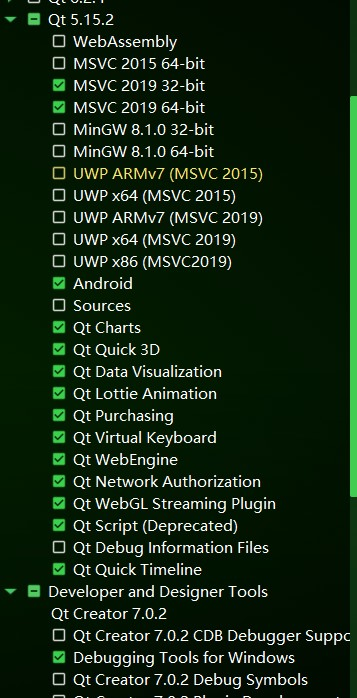
\includegraphics{我的QT安装配置.jpg}
\caption{我的QT安装配置} \label{fig:我的QT安装配置}
\end{figure}

选择\colorbox{LetMeFlyGray}{Qt5.15.2}是因为\colorbox{LetMeFlyGray}{5.15.2}是长期维护版本(\colorbox{LetMeFlyGray}{LTS})

选择\colorbox{LetMeFlyGray}{MSVC 2019 xx-bit}是因为我电脑上装有\colorbox{LetMeFlyGray}{Visual Studio}(\colorbox{LetMeFlyGray}{VS})并且我习惯于用\colorbox{LetMeFlyGray}{VS}开发\colorbox{LetMeFlyGray}{QT}程序。

选择\colorbox{LetMeFlyGray}{Android}是因为我想尝试使用QT开发安卓应用

像\colorbox{LetMeFlyGray}{Qt Charts}、\colorbox{LetMeFlyGray}{Qt Quick 3D}这些,都是QT中一些不错的功能。并且所占用体积并不大,因此我也选择了它们。

\subsubsection{在VS中安装QT插件}

QT插件的安装地址为\url{https://mirrors.tuna.tsinghua.edu.cn/qt/official_releases/vsaddin/2.8.1/}

下载下来直接双击即可安装。

安装完成后重启VS,点击选择\colorbox{LetMeFlyGray}{拓展 -> Qt VS Tools -> Options}

\begin{figure}[H]
\small
\centering
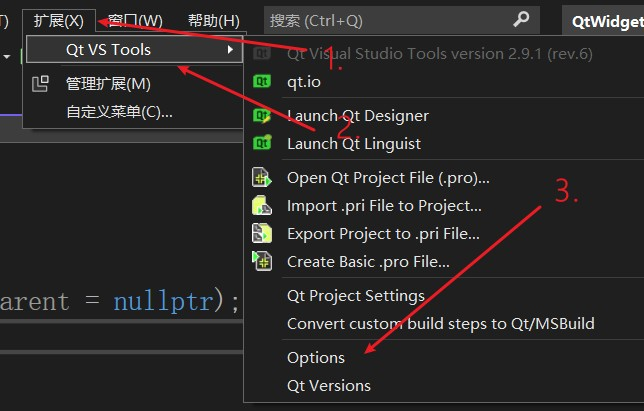
\includegraphics{拓展 - Qt VS Tools - Options.jpg}
\caption{拓展 - Qt VS Tools - Options} \label{fig:拓展 - Qt VS Tools - Options}
\end{figure}

选择\colorbox{LetMeFlyGray}{Qt -> Versions -> <add new Qt version> -> [资源管理器图标]}

\begin{figure}[H]
\small
\centering
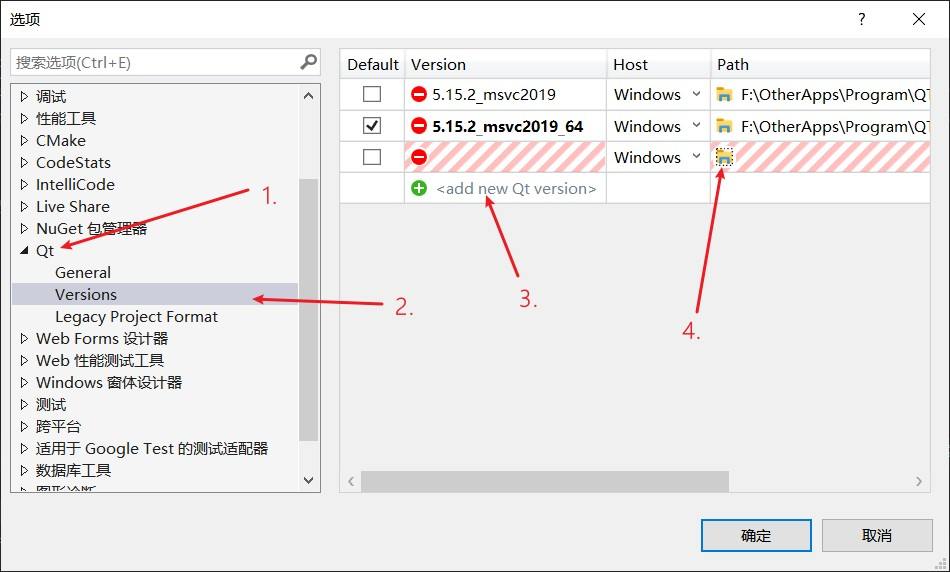
\includegraphics[width=\textwidth]{Qt - Versions - add new Qt version - [资源管理器图标].jpg}
\caption{Qt -> Versions -> <add new Qt version> -> [资源管理器图标]} \label{fig:Qt -> Versions -> <add new Qt version> -> [资源管理器图标]}
\end{figure}

在弹出的\colorbox{LetMeFlyGray}{资源管理器}中选择你所选择的\colorbox{LetMeFlyGray}{VS}的编译器的路径。

\begin{figure}[H]
\small
\centering
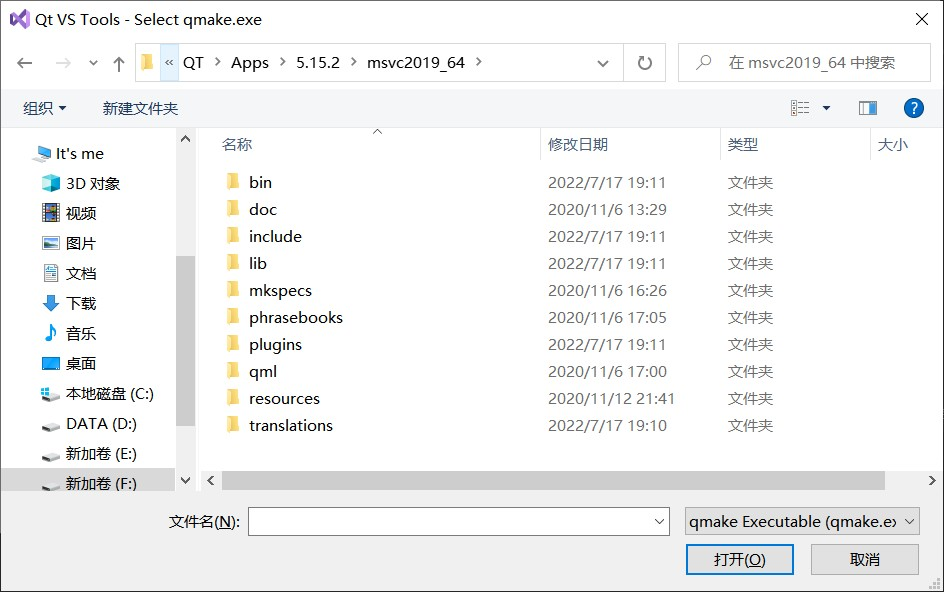
\includegraphics[width=\textwidth]{路径选择.jpg}
\caption{路径选择} \label{fig:路径选择}
\end{figure}

路径为:\colorbox{LetMeFlyGray}{QT安装位置 + QT版本 + msvc20xx + \\bin\\qmake.exe}

例如我的QT安装路径为:\colorbox{LetMeFlyGray}{F:\\OtherApps\\Program\\QT\\Apps},QT版本为\colorbox{LetMeFlyGray}{5.15.2}

\begin{figure}[H]
\small
\centering
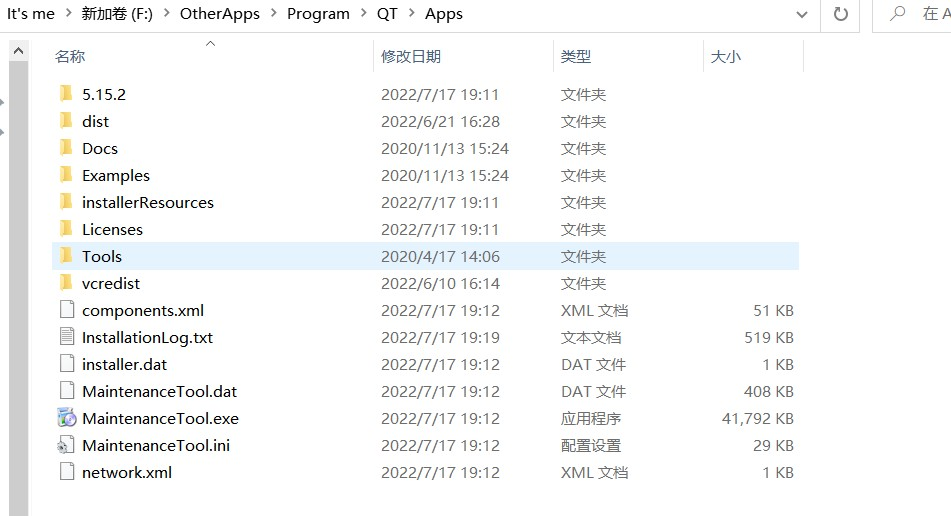
\includegraphics[width=\textwidth]{安装路径截图.jpg}
\caption{安装路径截图} \label{fig:安装路径截图}
\end{figure}

MSVC编译器的版本为\colorbox{LetMeFlyGray}{2019}的\colorbox{LetMeFlyGray}{64位}

则最终路径为\colorbox{LetMeFlyGray}{F:/OtherApps/Program/QT/Apps/5.15.2/msvc2019\_64/bin/qmake.exe}

你可以添加多个版本的编译器,添加完后可以选择一个默认的编译器,然后点击确定即可。

\begin{figure}[H]
\small
\centering
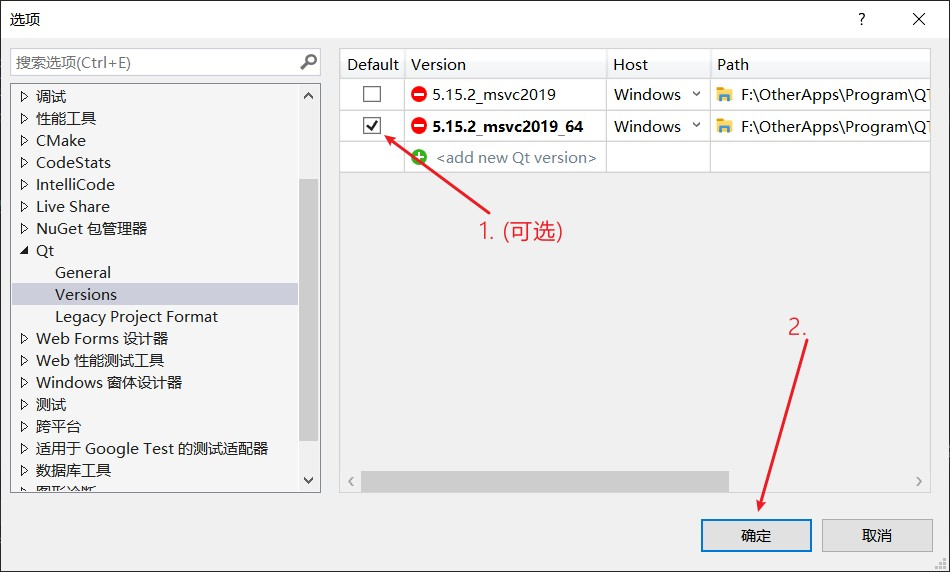
\includegraphics[width=\textwidth]{默认版本+点击确定.jpg}
\caption{默认版本 / 点击确定} \label{fig:默认版本+点击确定}
\end{figure}

\subsection{使用VS创建QT项目并运行}

打开VS,点击创建新项目

\begin{figure}[H]
\small
\centering
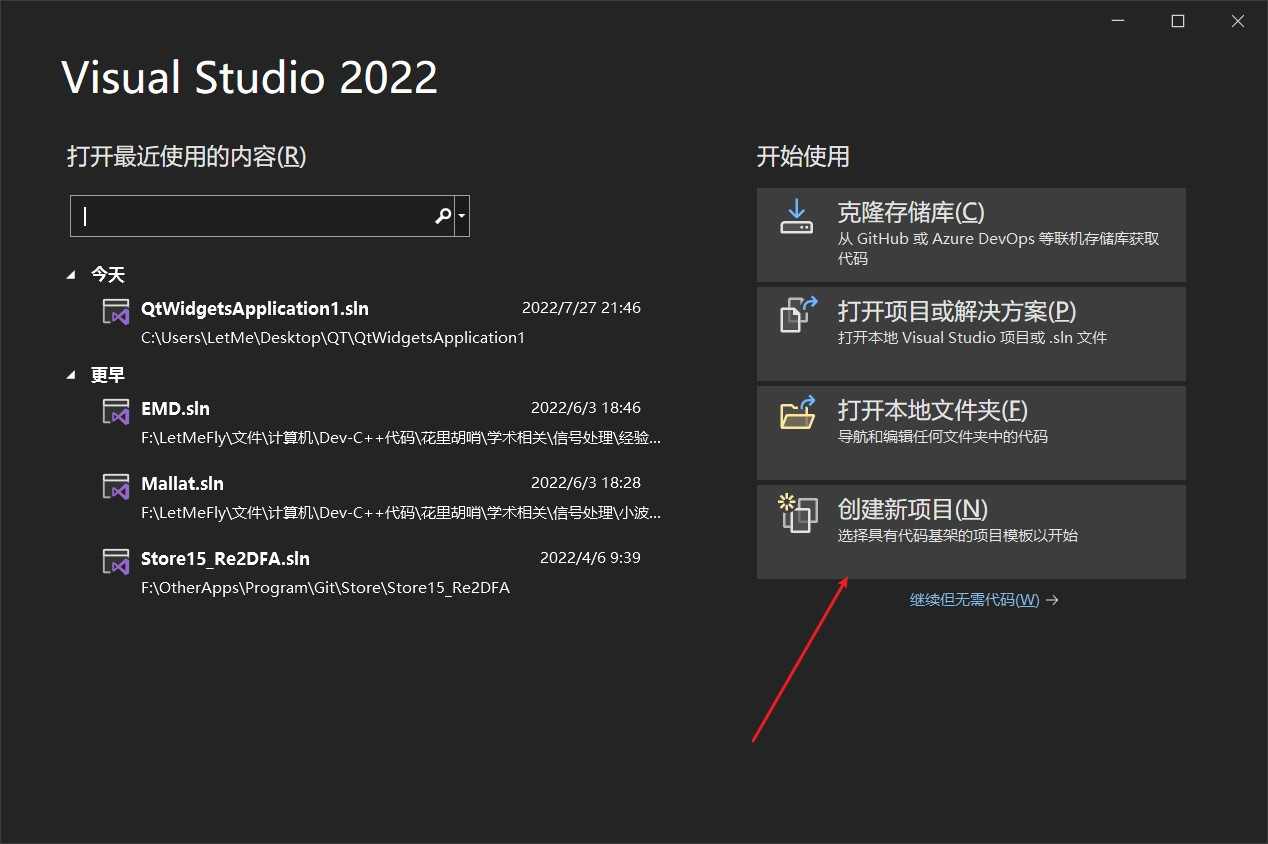
\includegraphics[width=\textwidth]{创建新项目.jpg}
\caption{创建新项目} \label{fig:创建新项目}
\end{figure}

如果要创建一般的图形界面,则可选择\colorbox{LetMeFlyGray}{Qt Widgets Application},然后点击\colorbox{LetMeFlyGray}{下一步}


\begin{figure}[H]
\small
\centering
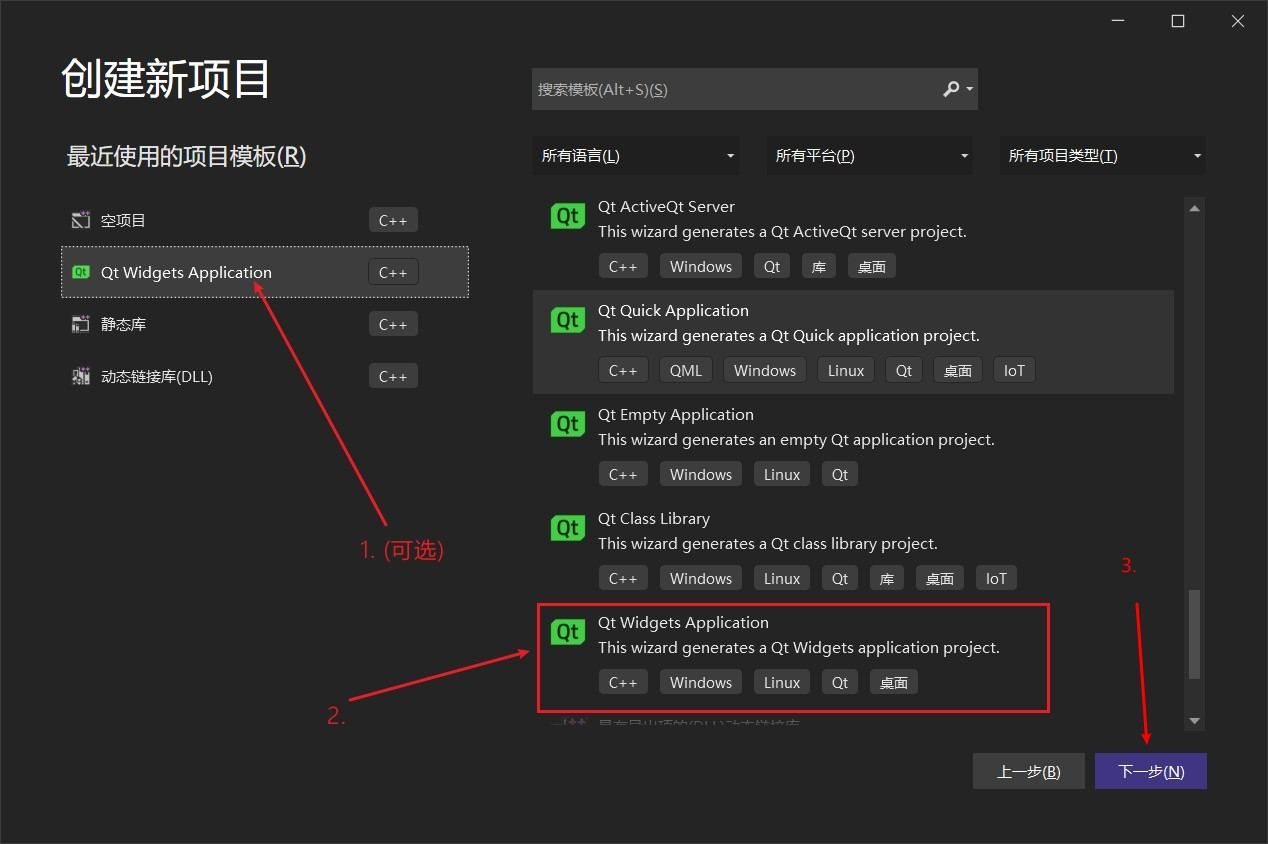
\includegraphics[width=\textwidth]{Qt Widgets Application.jpg}
\caption{Qt Widgets Application} \label{fig:Qt Widgets Application}
\end{figure}

设置项目名称、项目路径,点击创建

\begin{figure}[H]
\small
\centering
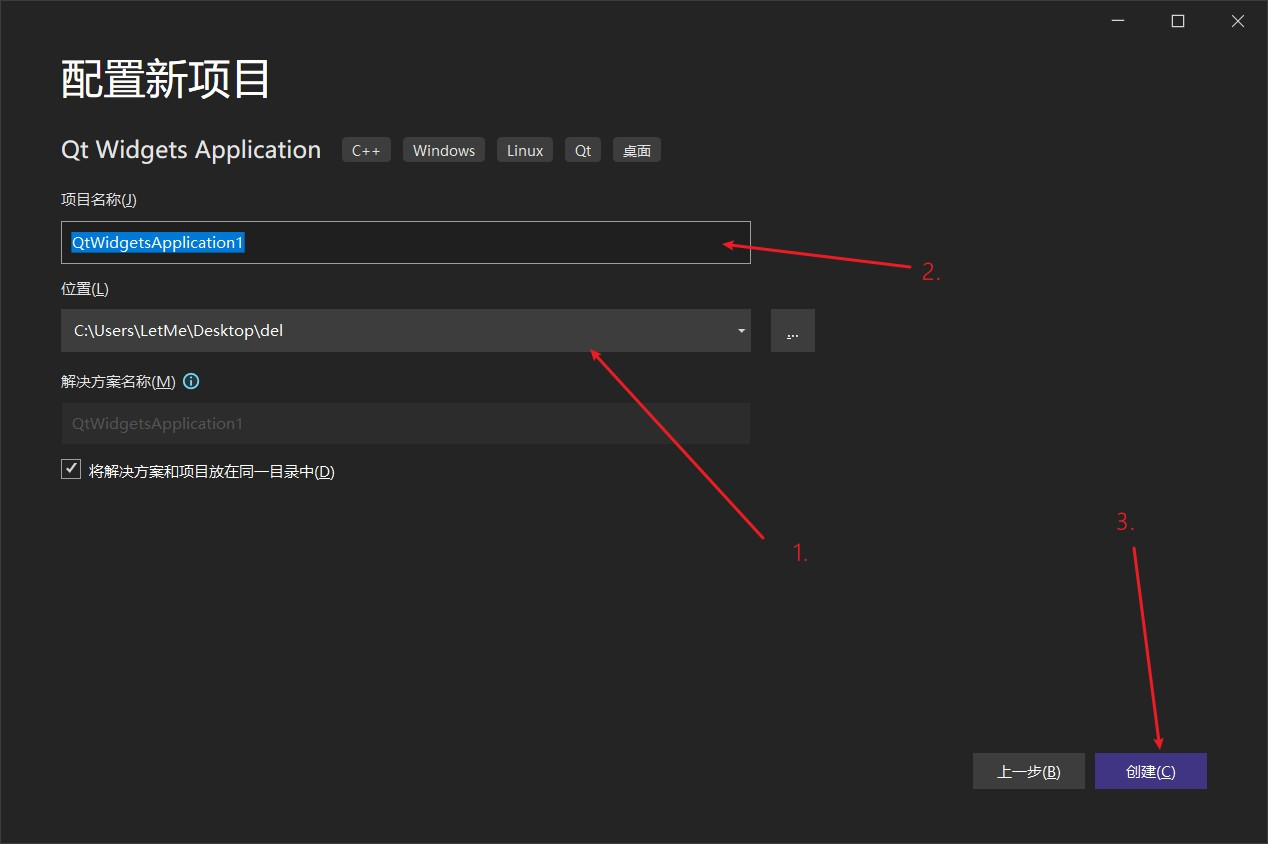
\includegraphics[width=\textwidth]{创建.jpg}
\caption{创建} \label{fig:创建}
\end{figure}

之后会跳出QT指引,基本上一路\colorbox{LetMeFlyGray}{next}最后\colorbox{LetMeFlyGray}{finish}即可

\begin{figure}[H]
\small
\centering
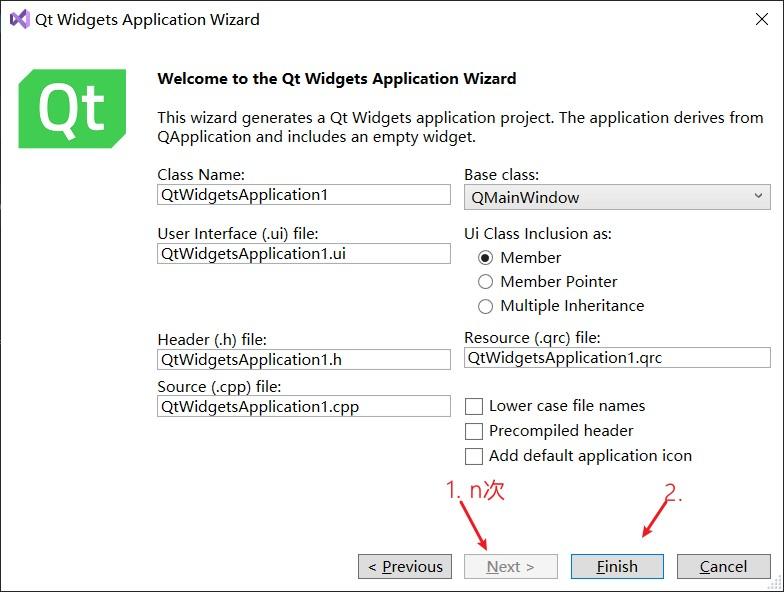
\includegraphics[width=\textwidth]{QT指引.jpg}
\caption{QT指引} \label{fig:QT指引}
\end{figure}

然后就可以愉快地进行Coding了。想要生成可执行文件,直接点击\colorbox{LetMeFlyGray}{本地 Windows 调试器}即可。

\begin{figure}[H]
\small
\centering
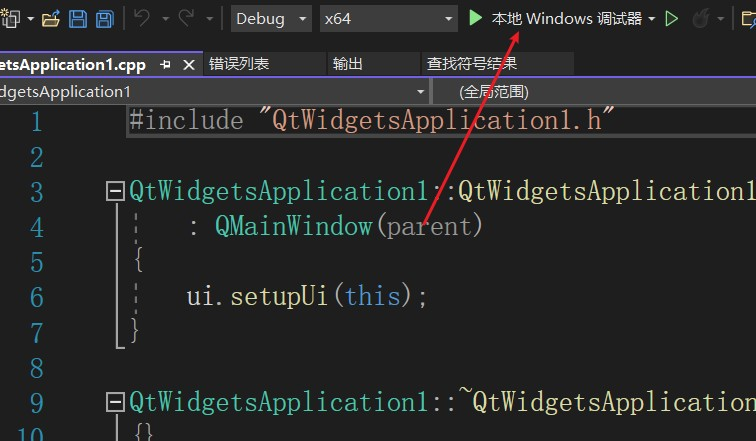
\includegraphics[width=\textwidth]{执行.jpg}
\caption{执行} \label{fig:执行}
\end{figure}

可以在右侧\colorbox{LetMeFlyGray}{解决方案资源管理器}中双击\colorbox{LetMeFlyGray}{.ui文件}进行布局设计

\begin{figure}[H]
\small
\centering
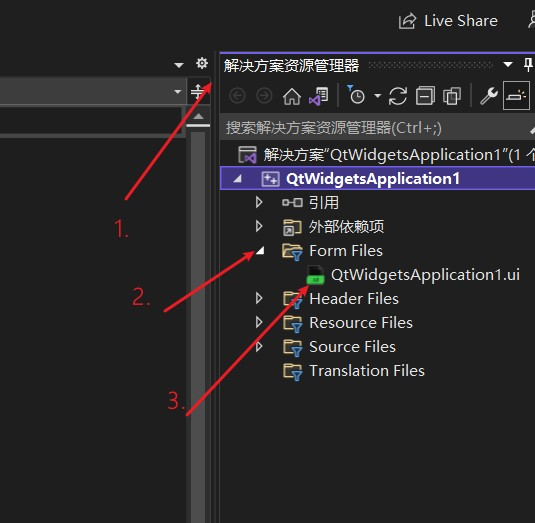
\includegraphics[width=\textwidth]{ui设计.jpg}
\caption{ui设计} \label{fig:ui设计}
\end{figure}

左侧直接拖拽就能进行界面设计

\begin{figure}[H]
\small
\centering
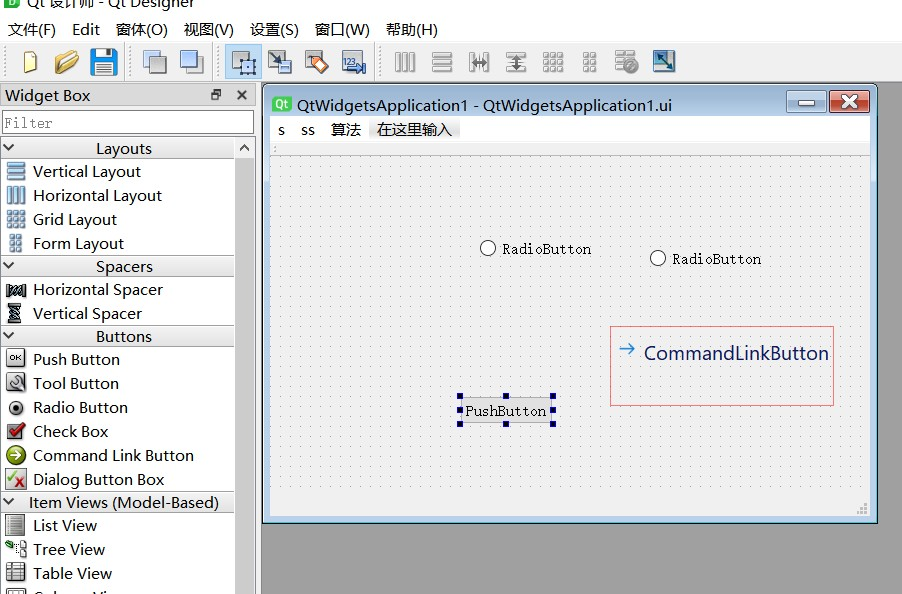
\includegraphics[width=\textwidth]{Designer.jpg}
\caption{Designer} \label{fig:Designer}
\end{figure}

\subsubsection{若VS中无法打开.ui进行设计}

直接在QtDesigner中编辑.ui文件可以很方便地进行布局。

但是如果VS出现了.ui文件打不开的情况,该怎么解决呢?

\begin{figure}[H]
\small
\centering
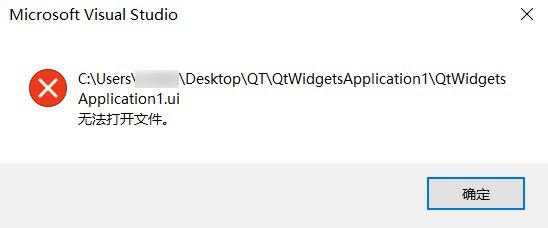
\includegraphics{无法打开.jpg}
\caption{无法打开} \label{fig:无法打开}
\end{figure}

在右侧解决方案管理器中,右键.ui文件,选择\colorbox{LetMeFlyGray}{打开方式}

\begin{figure}[H]
\small
\centering
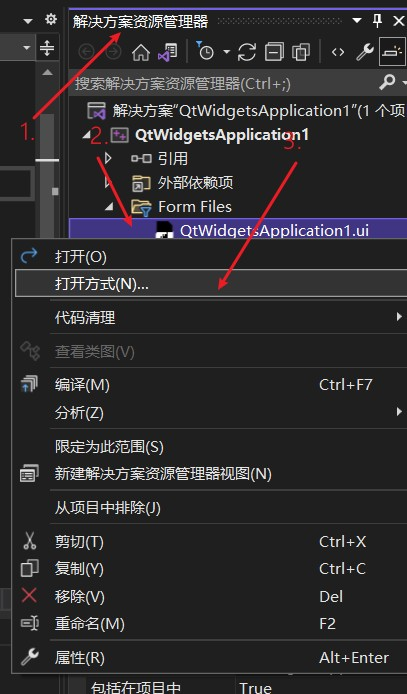
\includegraphics{打开方式.jpg}
\caption{打开方式} \label{fig:打开方式}
\end{figure}

\colorbox{LetMeFlyGray}{添加 -> 输入程序路径(你所选择的VS编译器对应目录下的designer.exe) -> 输入一个名字(你自己随便起一个) -> 点击确定}

\begin{figure}[H]
\small
\centering
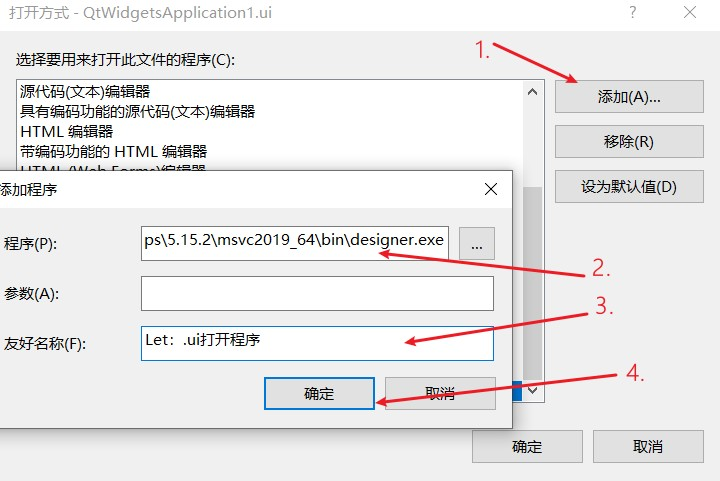
\includegraphics{新建打开方式.jpg}
\caption{新建打开方式} \label{fig:新建打开方式}
\end{figure}

然后选中刚才新创建的打开方式,点击设为\colorbox{LetMeFlyGray}{默认值}

\begin{figure}[H]
\small
\centering
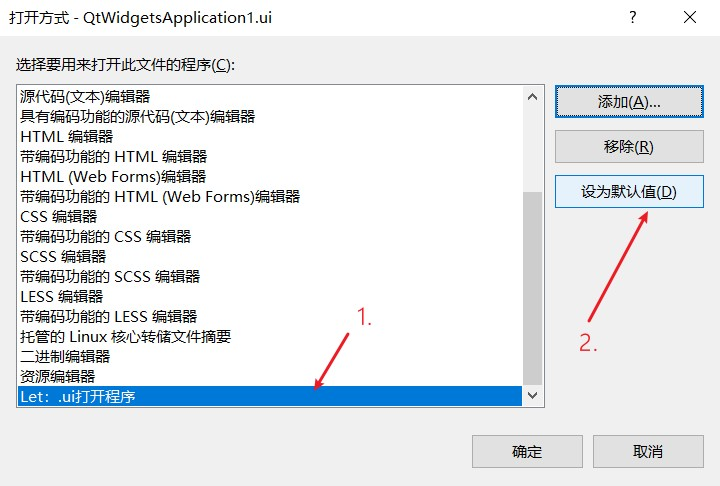
\includegraphics{设为默认打开方式.jpg}
\caption{设为默认打开方式} \label{fig:设为默认打开方式}
\end{figure}

然后,再双击\colorbox{LetMeFlyGray}{.ui文件}即可成功打开并编辑。

\subsection{控件、布局等}

\subsubsection{布局}

\begin{table}[H]
\caption{ 布局控件-功能表}
\centering
\begin{tabular}{r|l}
\toprule
布局控件 & 功能\\
\midrule[2pt]
Vertical Layout & 垂直方向上布局,组件自动在垂直方向上分布\\
Horizontal Layout & 水平方向上布局,组件自动在水平方向上分布\\
Grid Layout & 网格状布局,网状布局大小改变时,每个网格的大小都改变\\
Form Layout & 窗体布局,与网格状布局类似,但是只有最右侧的一列网格会改变大小\\
Horizontal Spacer & 一个用于水平分隔的空格\\
Vertical Spacer & 一个用于垂直分隔的空格\\
\bottomrule
\end{tabular}
\end{table}

\subsubsection{控件}

\subsubsubsection{窗口}

\textbf{窗口大小}

\begin{lstlisting}[language={c++},
    numbers=left,
    numberstyle=\tiny\monaco,
    basicstyle=\footnotesize\monaco]
myWidget::myWidget(QWidget *parent) : QWidget(parent) {
    resize(800, 600);  // 调整窗口大小
    setFixedSize(800, 600);  // 设置窗口固定大小(不和拉伸)
}
\end{lstlisting}

\textbf{窗口标题}

可以先show再改标题

\begin{lstlisting}[language={c++},
    numbers=left,
    numberstyle=\tiny\monaco,
    basicstyle=\footnotesize\monaco]
setWindowTitle("QT..");
\end{lstlisting}

\subsubsubsection{按钮}

\textbf{按钮Parent、文字}


\begin{lstlisting}[language={c++},
    numbers=left,
    numberstyle=\tiny\monaco,
    basicstyle=\footnotesize\monaco]
#include <QPushButton>
myWidget::myWidget(QWidget *parent) : QWidget(parent) {
    QPushButton *btn = new QPushButton("按钮", this);
    QPushButton *btn_withoutInit = new QPushButton();
    btn_withoutInit->setParent(this);
    btn_withoutInit->setText("按钮");
}
\end{lstlisting}

\subsubsection{控件的构造与析构}

关闭窗口则窗口对象会自动析构。

子控件添加parent时父控件也会同时将子控件添加到childrens中。因此当parent析构时也会自动调用子控件的析构函数。

\subsubsection{坐标}

\begin{lstlisting}[numbers=left,
    numberstyle=\tiny\monaco,
    basicstyle=\footnotesize\monaco]
O--------->x
|
|
↓
y
\end{lstlisting}

% 这里“↓”乱码我也不知道怎么整

\subsubsection{代码}

main:

\begin{lstlisting}[language={c++},
    numbers=left,
    numberstyle=\tiny\monaco,
    basicstyle=\footnotesize\monaco]
#include "Re2DFA.h"
#include <QtWidgets/QApplication>

int main(int argc, char *argv[])
{
    QApplication a(argc, argv);  // QApplication 用来创建一个应用程序类,必须要有,且只能有一个
    Re2DFA w;  // 这个是自定义的窗口类
    w.show();
    return a.exec();  // 应用程序进入消息循环
}
\end{lstlisting}

\subsubsection{中文乱码}

\begin{lstlisting}[language={c++},
    numbers=left,
    numberstyle=\tiny\monaco,
    basicstyle=\footnotesize\monaco]
#ifdef WIN32  
#pragma execution_character_set("utf-8")  
#endif
\end{lstlisting}

\subsubsection{文字换行}

QT Designer中设置\colorbox{LetMeFlyGray}{wordWrap}为true

\section{EEG信号处理笔记}

\subsection{名词解释}

\begin{enumerate} 
    \item DoA: Depth of anaesthesia(麻醉深度)
    \item EEG: electroencephalography(脑电图学)
    \item EMD: empirical mode decomposition(经验模态分解)
    \item HHT: Hilbert–Huang transform(希尔伯特-黄变换)
    \item HT: Hilbert transform(希尔伯特变换)
    \item IMF: intrinsic mode functions(固有模态函数)
    \item SampEn: sample entropy(样本熵)
    \item BIS: bispectral index(脑电双频指数)
    \item ECG: electrocardiography(心电描记术)
    \item FFT: Fast Fourier Transform(快速傅里叶变换)
    \item AUC ratio of α + β waves: area ratio of α + β waves (8–32 Hz) 
    \item EMG: electromyography(肌电图描记法)
    \item EOG: electrooculography(眼动电图描记法)
    \item ESUs: electrosurgical units(电外科装置)
    \item IFFT: Inverse fast Fourier transform(快速傅里叶逆变换)
    \item ApEn: approximate entropy(近似熵)
\end{enumerate}

\subsection{时域和频域}

时域是客观世界中唯一实际存在域;频域是一个数学构造,也被一些学者称为上帝视角。

\subsubsection{时域}

以时间轴为坐标表示动态信号的关系

\subsubsection{频域}

正弦波是频域中唯一存在的波形

\subsubsection{转换}

动态信号从时间域变换到频率域主要通过傅立叶级数和傅立叶变换实现。周期信号靠傅立叶级数,非周期信号靠傅立叶变换。时域越宽,频域越短。

\subsection{傅里叶变换}

傅里叶变换是从另一种角度看问题的方法。

信号大多是从时域度量的。傅里叶提出,任何周期性函数都可以由数个正弦函数叠加而成。

因此,可以将原始信号分解成数个正弦波的叠加。

对于一个正弦波,只需要直到其相位、频率、周期、振幅,就能确定这个波。

这就是频域的角度。

\begin{figure}[H]
\small
\centering
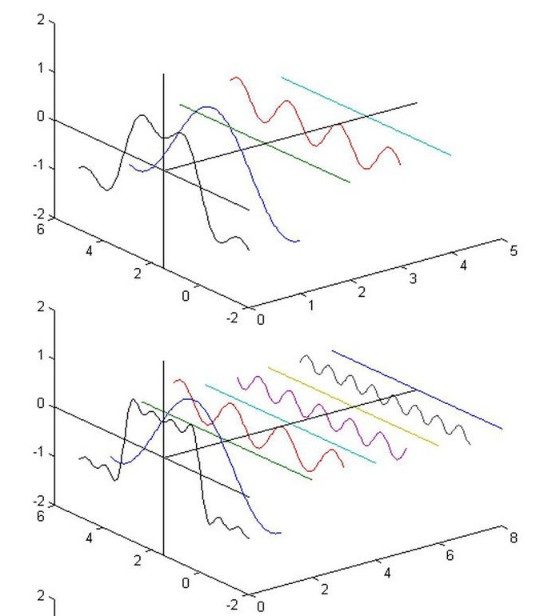
\includegraphics{傅里叶变换.jpg}
\caption{傅里叶变换} \label{fig:傅里叶变换}
\end{figure}

\subsection{经验模态分解}

经验模态分解,根据自身尺度进行分解。

$$x(t)=\sum_{i=1}^{n} c_{i}(t)+r_{n}(t)$$

$x(t)$是时域下的原始信号,$c_i(t)$是第$i$个IMF(固有模态函数),$r_n(t)$是残余信号。

\subsection{人脑信号}

人脑产生的脑电信号的正常频率在0.5赫兹Hz到32Hz之间,它们分别包含从低频到高频的$\delta$,$\theta$,$\alpha$波和$\beta$波。

$\delta$ (0.5–4 Hz), $\theta$ (4–8 Hz), $\alpha$ (8–16 Hz), $\beta$ (16–32 Hz)

其他频率的基本上都是噪声。

%===参考文献===
%\addcontentsline{toc}{section}{参考文献}
%\bibliographystyle{abbrv}     %论文引用格式
%\bibliography{E:/studio/wrtex/wrtkit/referbib/wholebiblio}
                         
\begin{thebibliography}{99}
\bibitem{A19}{\em \color{red}d2l.ai}. \url{https://zh.d2l.ai/}, 2022.
\bibitem{A19}{\em \color{red}百度百科:EEG}. \href{https://baike.baidu.com/item/%E8%84%91%E7%94%B5%E6%B3%A2/1599805}{https://baike.baidu.com/item/脑电波/1599805}, 2022.
\bibitem{A19}{\em Mu-Tzu Shih, Faiyaz Doctor, Shou-Zen Fan, Kuo-Kuang Jen and Jiann-Shing Shieh.  \href{https://www.mdpi.com/1099-4300/17/3/928}{\color{red}Instantaneous 3D EEG Signal Analysis Based on Empirical Mode Decomposition and the Hilbert–Huang Transform Applied to Depth of Anaesthesia}}, 2022.
\bibitem{A19}{\em \color{red}百度百科:傅里叶变换}. \href{https://baike.baidu.com/item/%E5%82%85%E9%87%8C%E5%8F%B6%E5%8F%98%E6%8D%A2/7119029}{https://baike.baidu.com/item/傅里叶变换/7119029}, 2022.
\bibitem{A19}{\em \color{red}百度百科:EMD}. \href{https://baike.baidu.com/item/EMD/3073860}{https://baike.baidu.com/item/EMD/3073860}, 2022.
\bibitem{A19}{\em \color{red}知乎:傅里叶分析之掐死教程}. \href{https://zhuanlan.zhihu.com/p/19763358}{https://zhuanlan.zhihu.com/p/19763358}, 2022.

\end{thebibliography}
\end{document}
%===结束===



History:
2022-8-20: 依据程勇老师的Note.tex创建;



